\documentclass[12pt,letterpaper,noanswers]{exam}
\usepackage[usenames,dvipsnames,svgnames,table]{xcolor}
\usepackage[margin=0.9in]{geometry}
\renewcommand{\familydefault}{\sfdefault}
\usepackage{multicol}
\usepackage{wrapfig}
\pagestyle{head}
\header{AM 22b Class 30}{}{Apr 13: Differential equations, p. \thepage}
\runningheadrule
\headrule
\usepackage{graphicx} % more modern
\usepackage{amsmath} 
\usepackage{amssymb} 
\usepackage{hyperref}
\usepackage{tcolorbox}
\usepackage[utf8]{inputenc}
\usepackage{diagbox}
\usepackage{graphicx} 
\usepackage{enumitem}
\usepackage{tikz}
\tikzstyle{startstop} = [rectangle, rounded corners, minimum width=3cm, minimum height=1cm,text centered, draw=black]

\tikzstyle{process} = [rectangle, minimum width=3cm, minimum height=1cm, text centered, draw=black, fill=gray!20]
\tikzstyle{decision} = [ellipse, minimum width=3cm, minimum height=0.5cm, text centered, draw=black, fill=white!30]
\tikzstyle{arrow} = [thick,->,>=stealth]
\usetikzlibrary{shapes.geometric, arrows}
\pagenumbering{arabic}

\usepackage[numbered,autolinebreaks,useliterate]{mcode}

\newcommand{\mb}[1]{\underline{#1}}

\begin{document}
 \pdfpageheight 11in 
  \pdfpagewidth 8.5in




% I need to review the torus trajectories...

\begin{itemize}
% \item There is a pre-class assignment (20 minutes of videos + a few WeBWorK exercises) due at 10am this Monday.  It is available on Canvas.
\itemsep0em
\item There is a skill check today (C27, 28, 29).  
\item There is a quiz this Friday (quiz 05).
\item Quiz 06 will be assigned the following Friday (Apr 23rd).
\item Sarah's Monday OH are cancelled this week.  (Tuesday and Wednesday OH are happening as scheduled).
\end{itemize}

\hrule
\vspace{0.2cm}

% partial derivatives, gradient
% local linearity, differential, directional deriv
% 2nd order partials + equations with partials

\noindent\textbf{Big picture}

We will learn how to analyze differential equations from three perspectives: using approximate solutions (slope fields + Euler's method + RK45), finding exact solutions (rarely, using separation of variables), using qualitative methods (identifying equilibrium solutions and whether they are `stable' or `unstable').

\vspace{0.2cm}
\hrule
\vspace{0.2cm}



\noindent\textbf{Skill Check C30 Practice}
\begin{questions}
\item Find all solutions to $\frac{dx}{dt} = x(1-x)$ where $x(t) = c$ with $c$ a constant (these are all of the equilibrium solutions).

\end{questions}

\noindent\textbf{Skill Check C30 Practice Solution}
\begin{questions}
\item $\frac{dx}{dt} = x(1-x) = 0$ when $ x = 0 $ or $1 - x = 0$ so $x(t) = 0$ is an equilibrium solution and $x(t) = 1$ is an equilibrium solution.
\end{questions}
\vspace{0.2cm}
\hrule
\vspace{0.2cm}

\noindent\textbf{Teams}

\begin{multicols}{2}

1.  student names
\end{multicols}


\vspace{0.2cm}
\hrule
\vspace{0.2cm}



% \noindent\textbf{Arclength} \S 18.1

% \noindent\textbf{Length of the siphonophore}

% The siphonophore pictured below is estimated to have a 49 foot diameter.  Based on what is visible in the image, how would you approximate its length?
% \vspace{2in}

% \begin{multicols}{2}
% 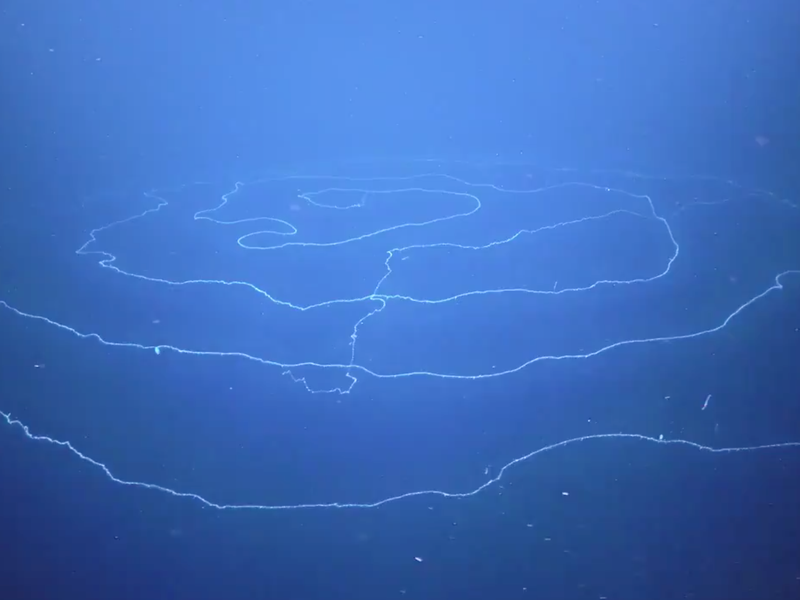
\includegraphics[width=0.45\textwidth]{img/C30p1.png}  

% ``This siphonophore may be the longest ever recorded. (Schmidt Ocean Institute)''
% {\color{blue}\hyperref[https://www.smithsonianmag.com/smart-news/giant-eerie-string-creature-hunting-food-indian-ocean-180974647/]{Click here for link to Smithsonian article}}.  Accessed 13 April 2020
% \end{multicols}



\noindent\textbf{Differential equations} \S 11.1
\begin{tcolorbox}
\begin{itemize}
\itemsep0em
    \item A \textbf{differential equation} is an equation that involves a derivative.
    \item An equation like $\cos x = 0$ has a family of solutions, $x = 2\pi n$ for $n\in \mathbb{Z}$ with each solution a single value of $x$.  A differential equation like $\dfrac{dx}{dt} = x$ has a family of solutions $x(t) = ce^t$ where each solution is a function.  
    \item A single differential equation can encode an entire family of solution curves $x(t)$.
    \item An \textbf{equilibrium solution} of a differential equation $\dfrac{dx}{dt} = f(x)$ is a solution $x(t) = c$ where the value of $x$ is constant for all times.  Such a solution must satisfy $f(c) = 0$ so that $\frac{dx}{dt} = 0$ (meaning that $x(t)$ does not change with time).
\end{itemize}
\end{tcolorbox}

\begin{tcolorbox}
\begin{itemize}
\itemsep0em
    \item A \textbf{differential equation} $\dfrac{dx}{dt} = f(x)$ can be thought of as a limit of a difference relationship $\dfrac{\Delta x}{\Delta t} = f(x)$.
    \item Many models are models of the rate of change of a quantity.  Such models would be encoded via a differential equation.
\end{itemize}
\end{tcolorbox}


\noindent\textbf{Example (population model)}

The population of the United States, $P$, has been measured every ten years since 1790 (via the decennial census).  Consider the following two models for $\Delta P/\Delta t$, the average change in the population per year during the ten year period between census measurements ($\Delta t = 10$).  Creating a model for the change in population is a way to predict the population at a future time.  What do you think of these models?  
\begin{enumerate}
\itemsep2em
    \item $\Delta P/\Delta t = c$ where $c$ is a constant.
    \item $\Delta P/\Delta t = a P$ where $a$ is a constant and $P$ is the population at the beginning of the ten years.
    \item Generate another model for $\Delta P$.
\end{enumerate}
\vspace{0.7in}


\noindent\textbf{Example (population model)}

Data from the decennial census is plotted below.  What is shown is $\dfrac{\Delta P/\Delta t}{P}$ where $\Delta P$ is the change in population from measurement $k$ to measurement $k+1$, $P$ is the population in measurement $k$ and $\Delta t$ is ten years.

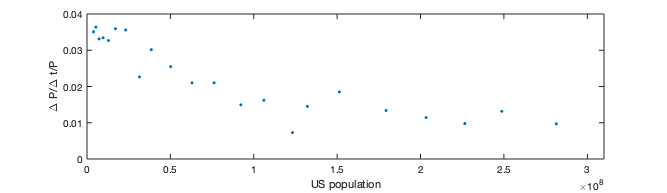
\includegraphics[width=\textwidth]{img/C29dpdtoverpvsp.png}

Two different models are plotted below
\begin{enumerate}
    \item $\frac{\Delta P/\Delta t}{P} = k$ (red line)
    \item $\frac{\Delta P/\Delta t}{P} = aP+b$ (black line)
\end{enumerate}

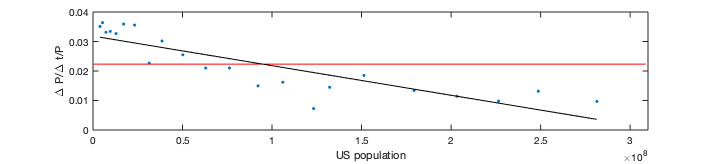
\includegraphics[width=\textwidth]{img/C29fitp2.png}

\vspace{0.2cm}
\hrule
\vspace{0.2cm}

\noindent\textbf{Equilbrium solutions}
\begin{enumerate}
\itemsep3em
    \item Find all solutions $P(t) = c$ such that $\dfrac{dP}{dt}$ remains at zero for $\dfrac{dP}{dt} = k P$.
    
    \item Find all solutions $P(t) = c$ such that $\dfrac{dP}{dt}$ remains at zero for $\dfrac{dP}{dt} = kP(b - P)$.
\end{enumerate}

\vspace{0.7in}

\vspace{0.2cm}
\hrule
\vspace{0.2cm}
\begin{tcolorbox}
\textbf{Euler's method} for approximating the solution to a first order initial value problem is an algorithmic method that is similar to finding an approximate solution using the graph of a slope field.  (For a slope field, $\frac{dy}{dx}$ is plotted vs $x$.)
\begin{enumerate}
    \item Choose your starting point, $x_0, y_0$ (the initial value).
    \item Use the differential equation to find the slope of the solution function, $y(x)$, at that point.
    \item Assume the slope of the solution function is constant for a small interval, $\Delta x$, of the independent variable.  \emph{This is a big assumption}.
    \item Find an approximation for a new point on the solution curve: $y_1 = y_0 + \left.\frac{dy}{dx}\right\vert_{x=x_0,y=y_0}\Delta x$.  $y_1 \approx y(x_0 + \Delta x)$.
    \item Let $x_1 = x+\Delta x$.  Use $x_1, y_1$ as your starting point and repeat the process to find $x_2, y_2$.
\end{enumerate}
The set of points $(x_k,y_k)$ form an approximation to the solution curve $y(x)$ where $\frac{dy}{dx}$ is given by the differential equation and $y(0) = x_0$.
\end{tcolorbox}

\noindent\textbf{Matlab interlude}

Open the file \texttt{USpopulation.m}.  Use Euler's method to approximate solutions for the two models above, then plot the approximate solutions against the Census data.  
\begin{enumerate}
    \item What do you think of these models and their predictions?
    \vspace{1in}

    \item If you were asked to provide a range of possible values for the US population in 2050 based on this Census data, how would you approach that?
        \vspace{1in}
        
\end{enumerate}





\vspace{0.2cm}
\hrule
\vspace{0.2cm}

% \noindent\textbf{Exponential growth vs logistic growth}

% \noindent\textbf{Example.  Exponential growth.} Consider the population model $\frac{dP}{dt} = kP$.  Identify the range of $P$ for which $\frac{dP}{dt}$ is positive, negative, or zero.
% \vspace{1in}

% \noindent\textbf{Example.  Logistic growth.} Consider the population model $\frac{dP}{dt} = kP(b - P)$.  Identify the range of $P$ for which $\frac{dP}{dt}$ is positive, negative, or zero.
% \vspace{1in}

% \noindent\textbf{Stability of an equilibrium solution}
% \begin{tcolorbox}
% \begin{itemize}
% \itemsep0em
%     \item 
% \end{itemize}
% \end{tcolorbox}



\noindent\textbf{Is the sum of two solutions also a solution?}
\begin{tcolorbox}
\begin{itemize}
\itemsep0em
    \item A \textbf{linear differential equation} is a differential equation of the form $f(x,\frac{dx}{dt}, \frac{d^2x}{dt^2}, ...) = 0$ where $f$ is a linear polynomial in $x$ and its derivatives.
    \begin{itemize}
        \itemsep0em
        \item Example: $\dfrac{d^2x}{dt^2} + 2\cos t \frac{dx}{dt} - 3t^3 x = 0$ is linear differential equation.
   \item  Non-example: $\dfrac{d^2x}{dt^2} + 2\cos t \frac{dx}{dt}x - 3t^3 x = 0$ is nonlinear differential equation.  \emph{$\frac{dx}{dt}x$ is nonlinear in $x$}.
    \end{itemize}
    \item A linear differential equation is called \textbf{homogeneous} when there are no constant terms in the equation.  
    \begin{itemize}
    \itemsep0em
        \item Example: $\dfrac{dx}{dt} - 3x = 0$ is homogeneous. 
   \item  Non-example: $\dfrac{dx}{dt} - 3x + 2 = 0$ is nonhomogeneous.
    \end{itemize}
\end{itemize}

\end{tcolorbox}

\noindent\textbf{Example: addition of solutions}.  

$\dfrac{dx}{dt} - t x = 0$ is a linear homogeneous differential equation.  Assume $x_1(t)$ is a solution of this equation.  Assume $x_2(t)$ is a solution as well.  Consider $x_3(t) = a_1x_1(t) + a_2x_2(t)$ for $a_1$ and $a_2$ constants.  Show that $x_3(t)$ is a solution of the differential equation.
\begin{enumerate}
    \item Given that $x_1(t)$ and $x_2(t)$ are solutions, write out mathematical statements satisfied by $x_1(t)$ and by $x_2(t)$.
    \vspace{1in}
    
    \item Use the statements you've written above to show that $\dfrac{d x_3}{dt} - t x_3 = 0$.
    \vspace{1in}
\end{enumerate}

\noindent\textbf{Example: no addition of solutions}.
$\dfrac{dx}{dt} - t x + 2 = 0$ is a linear nonhomogeneous differential equation.  Assume $x_1(t)$ is a solution of this equation.  Assume $x_2(t)$ is a solution as well.  Consider $x_3(t) = a_1x_1(t) + a_2x_2(t)$ for $a_1$ and $a_2$ constants.  How does the argument you used above break down when you try to show that $x_3(t)$ is a solution?
\vspace{2in}

\noindent\textbf{Example: no addition of solutions}.
$\dfrac{dx}{dt} - t x^2 = 0$ is a nonlinear differential equation. \emph{$x^2$ is nonlinear in $x$}.  Assume $x_1(t)$ is a solution of this equation.  Assume $x_2(t)$ is a solution as well.  Consider $x_3(t) = a_1x_1(t) + a_2x_2(t)$ for $a_1$ and $a_2$ constants.  How does the argument you used above break down when you try to show that $x_3(t)$ is a solution?
\vspace{2in}




\vspace{0.2cm}
\hrule
\vspace{0.2cm}


\end{document}